% \documentclass[aps,noshowpacs,superscriptaddress,nofootinbib,notitlepage]{revtex4-1}

% \documentclass[a4paper,10pt]{article}
% \usepackage[utf8]{inputenc}
% \usepackage{graphicx}

% \title{Parity and Time Reversal Violation in Electron Scattering}
% \author{ \textbf{S.K. Singh} \\ \textit{ Aligarh Muslim University, Aligarh, India}}

% \begin{document}

% \maketitle

% \begin{abstract}

% \end{abstract}

\documentclass[aps,noshowpacs,superscriptaddress,nofootinbib,notitlepage]{revtex4-1}

\usepackage{graphicx}% Include figure files
\usepackage{braket} 
\usepackage{float}%
\usepackage{amsmath}
 \usepackage{bbold} % for identity matrix 
 \usepackage[normalem]{ulem} % for strike through text 

\usepackage{diagbox}


\usepackage[usenames, dvipsnames]{color}
 

\usepackage[colorlinks]{hyperref}  

% Puts a slash through a character
\def\slashchar#1{\setbox0=\hbox{$#1$}
   \dimen0=\wd0 \setbox1=\hbox{/} \dimen1=\wd1
   \ifdim\dimen0>\dimen1 \rlap{\hbox to \dimen0{\hfil/\hfil}} #1
   \else  \rlap{\hbox to \dimen1{\hfil$#1$\hfil}} / \fi}
\def\p{\slashchar{p}}
\def\q{\slashchar{q}}
\def\D{\slashchar{D}}
\graphicspath{{./plots/}}

\begin{document}

\title{Parity and Time Reversal Violation in Electron Scattering}

\author{S. K.  \surname{Singh}}
\affiliation{Department of Physics, Aligarh Muslim University, Aligarh-202 002, India} 

\begin{abstract} 
The physical process of the electron scattering from nucleons and nuclei are P and T conserving as hey are governed by the electromagnetic interactions. However in the presence of the weak neutral current in the electron sector as predicted by the Standard Model,some polarization and spin dependent observables involving the electrons and nucleons in the final state are induced which violate P and T invariance.A summary of theoretical and experimental work done on such observables is presented.
\end{abstract}

% \pacs{25.30.Pt,13.15.+g,12.15.-y,12.39.Fe}
\maketitle

\section{Foreword}
It is matter of great pleasure for me to be invited to contribute to the commemorative volume going to be published in honor of Prof. G. Ramachandran.  Although I did not get enough opportunity to have short range interactions with him, his work on polarization observables in various reactions induced by the photons and the electrons in nuclear targets brought me in academic contact with him when I got interested in studying the parity violating effects in electron scattering induced by the neutral currents (NC) in weak interactions. The neutral currents (NC) were already observed at CERN in neutrino interactions in 1973~\cite{Hasert:1973ff} which confirmed the Standard Model (SM) of electro-weak interactions~\cite{Weinberg:1967tq,Salam:1968rm}. The Standard Model also predicted the neutral currents in the electron sector.  Consequently, a great interest was generated in studying various effects like the polarization observables and other  spin dependent effects induced by the weak  neutral currents in electron scattering which were observed in 1978~\cite{Prescott:1978tm,Prescott:1979dh}. In the Standard Model such effects were predicted to be  larger from neutron as compared to the proton targets, thus focusing on electron scattering from   deuteron and other nuclear targets which started my interest in pursuing the study of such effects in electron scattering from nuclei.  As an young researcher it was natural to think of collaborating with Prof. Ramachandran and learning various methods in  spin physics from him and apply them to study the P and T violating polarization observables in electron scattering from nuclear targets. 

   Our first collaboration was to calculate the  non vanishing vector polarization of recoil deuteron in the elastic electron  deuteron   scattering in the presence of the weak neutral currents~\cite{Ramachandran:1978zz} which led to the opportunities for our further collaboration in this field and also my trip to Mysore University  to visit him to discuss various aspects of spin physics and its applications to the electron scattering in order to study the implications of the weak neutral current  in electron scattering. Prof. MVN Murthy, a young energetic student working with Prof. Ramachandran at that time was an excellent collaborator to help us in understanding many physics issues and doing numerical computations which helped us in writing many papers in collaboration in the subject~\cite{Murthy:1979ws,Singh:1980xi,Murthy:1983wt} and also extending our collaboration to study some processes on nuclear  photo-production of pions~\cite{Murthy:1982fe}. The methods of spin physics learned during this period were very useful later when I came back to this field again to study the polarization observables in electron scattering as well as in neutrino scattering from nucleons and nuclear targets which can be used to test the Parity(P) and Time Reversal Invariance (TRI) in these processes~\cite{Arenhovel:2000if,Ahmad:2008zs,Akbar:2017qsf,Fatima:2018gjy,Fatima:2018tzs}.
  \section{Introduction}
   The study of discrete symmetries like Parity and Time Reversal have played an important role in the development of weak interactions theory leading to the unification of weak and electromagnetic interactions formulated in the standard model. The experimental confirmation of the existence of neutral current in the neutrino sector at CERN and later in the electron sector at SLAC in accordance with the predictions of the Standard Model  established it as the unified theory of weak and electromagnetic interactions.  The observations of the parity violating  asymmetries and the polarization observables in the scattering of polarized electron from  hadronic targets in the elastic,  inelastic and deep inelastic  scattering have been the important   milestones in establishing the Standard Model  as the unified theory of electroweak interactions  of  leptons and hadrons.  The parity violating effects observed in various physical processes relevant in atomic physics,  nuclear physics and particle physics are found to be consistent with  predictions of Standard Model except in very few cases where a decisive comparison with the experiments with  enhanced  precision and improved theoretical calculations require a better knowledge of  understanding atomic and/or nuclear physics~\cite{Athar:1970esm}.
   
   On the other hand, the time reversal invariance (TRI) has been observed to be violated only in K and B decays and there is no evidence of T  violation in the  lepton sector  involving neutrinos and/or  electrons.  Recently an experiment looking for CP  violation ( equivalent to T    violation assuming CPT symmetry) performed with neutrinos and antineutrino at JPARC  is  interpreted as the first indication that T (CP) may be violated in the neutrino sector~\cite{nature}. However,  there seems to be no attempts in recent days to look for T  violation  in electron scattering except for some old experiments done at SLAC~\cite{Prepost:1968bow,Rock:1970sj}. Nevertheless, theoretically there have been some attempts in literature to discuss various  observables involving neutrinos and electrons which may provide information about the status of T  invariance in the lepton  sector  \cite{Ramachandran:1967vci,Frederico:1991vb,Fatima:2018gjy,Fatima:2018tzs}. 
   
   
     In this contribution,  I discuss some of the major  attempts to study the role of the physics of polarization observables and spin correlations, a subject dear to Prof. Ramachandran in describing the present status of Parity and Time Reversal Violation in electron scattering.
     \section{Parity violation in electron scattering}
     The physical process of electron scattering is parity conserving and takes place through one photon exchange which is described in the second order perturbation theory using the interaction Lagrangian density for electromagnetic interaction  of charged particles ${\cal L}_{int}^{em}$  given by 
     \begin{equation}
     {\cal L}_{int}^{em}(x) = -e j_{\mu}^{e}(x)A^{\mu}(x),
     \end{equation}
     where $A_\mu(x)$ is the electromagnetic potential and $j_\mu^e(x)$ is the electromagnetic current of a particle with charge e and is given by 
     \begin{equation}
     j_\mu =\bar{\psi_l}\gamma_\mu \psi_l(x)
     \end{equation}
     for particles of spin $\frac{1}{2}$ like electrons and quarks described by the Dirac field $\psi(x)$. The matrix elements and cross sections are calculated using the Feynman diagrams shown in the Fig.~\ref{Fig:1} which gives the non-vanishing contribution in the lowest order.
     \begin{figure}
      \begin{center}
    %   \includegraphics[width=4in, height=1.5in]{fig1.eps}
      \includegraphics[scale=0.6]{fig1.eps}
      \caption{Elastic e-p scattering with exchange of photon($\gamma$) and neutral gauge boson(Z).}
      \label{Fig:1}
    \end{center}
    \end{figure}
     The matrix element corresponding to this diagram in the lowest order is written in momentum space as:
     \begin{equation}
     {\cal M}^{\gamma} = -\frac{e^2}{q^2}\bar{u}_l(k^\prime)\gamma^\mu u_l(k) \bar{u}(p^\prime)J_\mu^\gamma u(p),
    \end{equation}
  where 
  \begin{equation}
   <p^\prime|J_\mu^\gamma|p>= \bar{u}(p^\prime)\big[F_1^{\gamma}(q^2)+i\frac{\sigma_\mu q^\nu}{2M}F_2^{\gamma}(q^2)\big]u(p) 
   \end{equation}
  and $F_1^\gamma(q^2),F_2^\gamma(q^2) $ are the Dirac-Pauli Form Factors of nucleons related with the Sachs electric and magnetic Form Factors $G_E^\gamma(q^2)$ and $G_M^\gamma(q^2)$  as follows
  \begin{equation}
  G_E^\gamma(q^2) = F_1^\gamma(q^2)+\frac{q^2}{4M^2}F^\gamma_2(q^2)
  \end{equation}
  
   \begin{equation}
   G_M^\gamma(q^2) = F_1^\gamma(q^2)+F_2^\gamma(q^2)
  \end{equation}
  with $F_1^p(0)=1, F_1^n(0)=0, F_2^p(0)=\mu_p$ and $F_2^n(0)=\mu_n$ used to define the $G_E^{p,n}(0)$ and $G_M^{p,n}(0)$. \\
  The momentum (q) dependence of the Form Factors $G_2^{p,n}(q^2)$ is parameterized by various authors in last 50 years, but the simplest and most popular parameterization is given by a dipole parameterization 
  \begin{align}
      G_E^p(q^2)=\frac{1}{(M_v^2 - q^2 )^2}  \quad ,  \quad 
      G_M^{p(n)}(q^2)=\frac{1+\mu_p(\mu_n)}{(M_v^2 - q^2)^2} ,
  \end{align} 
  with $M_v= 0.84$GeV and $\lambda_n=5.6$\\
 The cross section is calculated for the electron proton scattering for electrons with initial and final energy E and $E^\prime$ and written as
  \begin{eqnarray}
  \frac{d\sigma}{d\Omega}= \frac{\alpha^2}{4E^2\sin^2\frac{\theta}{2}}\Big\lbrace\frac{{G_E^P}^{2}+{G_M^P}^{2}}{1+\tau} \cos^2\frac{\theta}{2}+2\tau {G_M^P}^{2}(q^2)\sin^2\frac{\theta}{2}\Big\rbrace
  \end{eqnarray}
  with $\tau=-\frac{q^2}{4M^2}$ and $q^2=-4EE^\prime \sin^2\frac{\theta}{2}$. 
  
The Standard Model of electroweak interactions predicts the existence of neutral currents  for the elementary particles like leptons and quarks which interact through exchange of Z  boson in addition to the weak charged current interacting through the exchange of $W^\pm$ bosons. While the exchange of $W^\pm$  gives the physical processes induced by weak interactions like $\beta$  decays, muon  capture and  quasi elastic $\nu(\bar{\nu})$  scattering from nucleons through the interaction Lagrangian known of the V-A theory.  In the neutral current sector,  the interaction Lagrangian for elementary fermions (f) like electrons (e) and quarks (q) are given by
\begin{equation}\label{Lezz}
{\cal L}_{int}^{eeZ}=\frac{g}{2\cos\theta_W}j_\mu^Z(e)Z^\mu
\end{equation}
\begin{equation}\label{Leqq}
{\cal L}_{int}^{qqZ}=\frac{g}{2\cos\theta_W}j_\mu^Z(e)Z^\mu
\end{equation}
where  \\
\begin{align}
    j_\mu^Z(e)&=\bar{e}\gamma_\mu(g_V^e-g_A^e\gamma_5)e \\ 
    j_\mu^Z(q)&=\bar{q}\gamma_\mu(g_V^q-g_A^q \gamma_5)q
\end{align} 
where the couplings $g_V^{e,q}$ and $g_A^{e,q}$ are given in the Table:~\ref{Tab:1} and $g^2=2\sqrt{2}G_F M_W^2, ~\frac{g^2}{\cos^2\theta_W}=2\sqrt{2}G_F M^2_Z$ .

\begin{table}
\begin{center}
\begin{tabular}{ |c|c|c|}\hline
 \diagbox{Particles}{Couplings}  &$g_V$&$g_A$\\\hline
electron (e) &$-\frac{1}{2}+2\sin^2\theta_W$&-$\frac{1}{2}$\\\hline 
up-quark (u) &$-\frac{1}{2}+\frac{4}{3}\sin^2\theta_W$&+$\frac{1}{2}$\\\hline
down-quark (d) &$-\frac{1}{2}+3\sin^2\theta_W$&-$\frac{1}{2}$\\\hline
 \end{tabular}
 \caption{Weak couplings for electrons and u,d quarks in Standard Model.}
 \label{Tab:1}
\end{center}
\end{table}


   \begin{figure}
  \begin{center}
      \includegraphics[width=4in, height=1.5in]{ee_eq.eps}
      \caption{Feynman diagrams for e-e and e-q scattering mediated by Z-bosons.}
      \label{Fig:ee-qq}
    \end{center}
    \end{figure}
   The interaction Lagrangian given in Eq.~\ref{Lezz} and \ref{Leqq} give rise to weak contribution to the e-e and e-q scattering in the second order of perturbation through the Feynman diagrams shown in Figure~\ref{Fig:ee-qq}. The neutral weak quark current $j^Z_\mu$ in Eq.~\ref{Leqq} is used to derive expression for the matrix element of the hadronic weak current between nucleons discussed in section.
   \begin{figure}
  \begin{center}
      \includegraphics[width=4in, height=1.5in]{fig2.eps}
      \caption{Inelastic electron scattering (a) $\vec{e}d\rightarrow\vec{e}np$ and (b) $\vec{e}p\rightarrow \vec{e}\Delta$.}
      \label{Fig:Delta}
    \end{center}
    \end{figure}
  
  The contribution of these diagrams to the  cross section is of the order of $\sim \big(\frac{g}{2\cos\theta_W}\big)^2 \approx \frac{1}{2}G_F^2$ i.e. the second order in the  Fermi coupling constant and is very small as compared to the dominant contribution from the electromagnetic scattering. They are effectively smaller by a factor $\approx \frac{G_F^2q^4}{\alpha^2}\approx 10^{-6}\big(\frac{q^2}{M^2}\big)$and are almost negligible. However the contribution to the cross section arising due to the interference between the electromagnetic and the weak terms would give rise to the parity violating effects due to the presence of axial vector current in the ${\cal L}_{int}^{eeZ}$and ${\cal L}_{int}^{qqZ}$ interaction and are of the order of $\frac{Gq^2}{\alpha M^2}\approx 10^{-3} \frac{q^2}{M^2}$. The experimental observations of such effects in various experiments performed with the polarized (unpolarized) electrons on unpolarized (polarized) electron (proton) , protons and other nuclear targets like $ ^4{He},^8{Be},^{12}{C}$ and $^{208}{Pb}$ have been the triumphs of the Standard Model. Specifically, the experiments on elastic electron- electron (Moller) scattering, elastic electron proton and electron nucleus scattering as well as the inelastic electron proton scattering leading to $\Delta$ excitation and the electro-disintegration of deuteron have been performed. Historically the first observation of the parity violation effects with electron beams was made in the deep inelastic scattering (DIS) of longitudinally polarized electron from deuteron targets at SLAC in which a left-right asymmetry was observed  in agreement with the prediction of Standard Model. Since then many experiments in the DIS regions  have been done at SLAC and JLAB. 
Most of these experiments observe a left-right asymmetry in the the scattering of polarized electron  from the electron and hadron targets defined as
\begin{equation}
{\cal A}= \frac{\sigma_R(q^2)-\sigma_L(q^2)}{\sigma_R(q^2)+\sigma_L(q^2)}
\end{equation}
where $\sigma_{R,L}(q^2)$ are the differential cross sections with the right and left handed electrons. On the other hand some experiments also observe the polarization transfer of electron or proton in the case of the scattering of polarized electron from polarized ( unpolarized) proton targets. Some of the polarization transfers and the double spin asymmetries are non zero even in the case of electromagnetic scattering which are parity conserving. However in the case of the parity violating double asymmetries and the polarization transfers it is possible to observe them as they are non zero in the presence of weak neutral currents of electron and/or protons. The polarization of final electron or proton of momentum $p^\prime$ is obtained by calculating the polarization vector $\xi^\alpha$ defined as 
\begin{equation}\label{eq:pol}
\xi^\alpha =\frac{Tr[\gamma^\alpha \gamma_5\rho_f(p^\prime)]}{Tr[ \rho_f(p^\prime)] } ,
\end{equation}

where $\rho_f(p^\prime)$ is spin density matrix  corresponding to the final fermion (electron or proton) of momentum $p^{\prime\mu}$ and is given by 
\begin{equation}
\rho_f(p^\prime)= L_{ \alpha \beta}(k,k^\prime)[Tr(\Lambda(p^\prime) )M^\alpha(p)\Lambda(p^\prime)\tilde{M}^\beta] ,
\end{equation}
where $L^{\mu \nu}(k,k^\prime)$ is the leptonic tensor: 
\begin{equation}\label{eq:lmunu}
    L_{\mu \nu}= 8 \left[  k_\mu  k^\prime_\nu  +  k_\nu  k^\prime_\mu  - g_{\mu \nu} k \cdot k^\prime 
    \pm  i \, \varepsilon_{\mu \nu \alpha \beta} k^\alpha {k^\prime \,}^\beta \right] \, ,
\end{equation}
with (lower)upper sign refers to the (anti-)neutrino. Our convention for the Levi-Civita tensor in four dimensions is 
$\varepsilon^{0123}=-\varepsilon_{0123}=1$. The $M_\alpha$ is the hadronic matrix element i.e. $M_\alpha=M_\alpha^\gamma+M_\alpha^Z$ and $\Lambda(p^\prime)$ is the projection operator of the fermion given by $\Lambda(p^\prime)=\not{p}^\prime+M$.

\subsection{Elastic Scattering}

The interference between contribution of one photon and Z- boson  exchange diagram shown in Fig.~\ref{Fig:moller}, the elastic scattering of longitudinally polarized electrons from nucleons and nuclei gives rise to left right asymmetry which is parity violating. 

The matrix elements corresponding to the above diagram are  written as 
\begin{eqnarray}
{\cal M}_\gamma= -\frac{e^2}{q^2}j^\mu_\gamma J_\mu^\gamma, ~~~~~~ {\cal M}_{Z}= -\frac{G_F}{\sqrt{2}}j_\mu^Z J^\mu_Z,
\end{eqnarray}
where
\begin{eqnarray}
j^\mu_\gamma&=& \bar{u}(k^\prime)\gamma^\mu u(k)\\
J^\mu_Z &=& \bar{u}(k^\prime)\gamma^\mu (g_V^e-g_A^e\gamma_5)u(k)
\end{eqnarray}
and 
\begin{eqnarray}\label{eq:curr}
J^{\gamma,Z}_\mu = \bar{u}(p^\prime)[F_1^{\gamma,Z}(q^2)\gamma_\mu+i\sigma_{\mu\nu}\frac{q^\nu}{2M}F_2^\gamma(q^2)+G_A^{\gamma,Z}(q^2)]u(p),
\end{eqnarray}
where $F_i^{\gamma,Z}(q^2)(i=1,2)$
are the Pauli-Dirac electromagnetic $(\gamma)$ and weak $(Z)$ vector form factors defined for protons and neutrons and are defined in terms of the Sachs electromagnetic and weak form factors of the nucleons $G^{\gamma,Z}_{E,M}(q^2)$ for protons and neutrons. Explicit expression of these form factors are given as
\begin{eqnarray}
 G_{E,M}^{Z(p,n)}&=&(1-4\sin^2 \theta_W)G_{E}^{\gamma(p,n)}(q^2)-G_{E,M}^{\gamma(n,p)} (q^2), \\
 G_A^{Z,p}(q^2)&=&-G_A^{Z,n}(q^2) \;\; = \;\; \frac{1}{2}G_A(q^2) \\ 
 G_A^{\gamma,p(n)}(q^2)&=& 0 . 
\end{eqnarray}
The $G^{\gamma,Z}_A(q^2)$ are the axial vector form factors for the nucleons with $G^{\gamma,p(n)}_A(q^2)=0$ for protons and neutrons and $G^{Z,p(n)}_Z(q^2)$ for nucleons satisfy $G^{Z,p}_A(q^2)=-G^{Z,n}_A(q^2)$. The Left-Right asymmetry ${\cal A}_{LR}$ defined in equation is then written as 
\begin{equation}
 {\cal A}_{LR}\propto \frac{Re|M^\gamma M_Z^*|}{|M_\gamma^2|+|M_Z^2|} \approx \frac{Re~ M^\gamma M_Z^*}{|M_\gamma^2|}
\end{equation}
 which is given by ${\cal A}_{LR}=-\frac{G_F Q^2}{4\sqrt{2}\pi\alpha}F^p(E_e,q^2)$ for proton target and $F^p(E_e,q^2)$ is given as
 \begin{equation}
F^p(E_e,q^2)= (A^{p}_E(q^2) +A_M^{p}(q^2)+A_A^p(q^2)).
 \end{equation}
The first two terms i.e. $A^{p}_E(q^2)$ and $A_M^{p}(q^2)$ describe the contribution from the interference between the electron axial vector current and nucleon vector current and the last term $A_A^p(q^2)$ is the interference between the electron vector current and nucleon axial vector current, the first being the dominant contribution. In the case of  iso-scalar targets like $^4{He}$, only the iso-scalar nucleon current contributes and the expression becomes very simple i.e. 
\begin{equation}
 {\cal A}_{LR} = \frac{G_F^2}{\pi\sqrt{2}\alpha}\sin^2\theta_W.
\end{equation}

There have been quite a few experiments done on various targets like proton, $^4{He}$ and $^{12}{C}$ with polarized electrons beam at MAINZ, MIT-Bates and JLAB during the last 20 years and the results are given in Table \ref{WS:asymm_tbl_elastic}~\cite{Erler:2014fqa}.
\begin{table}
\begin{center}
\begin{tabular}{|c|c|} \hline
 Experiment  & ${\cal A}_{LR}$ Elastic\\ \hline
 Mainz& $-9.4\pm20\%$ \\ \hline
 Mainz--A4&$-17.2\pm 5\%$ \\ \hline
 MIT--Bates& $1.62\pm 24\%$\\ \hline
 SAMPLE& $-5.61\pm 20\%$ \\ \hline
HAPPEX& $-15.05\pm 7.5\%$\\ \hline
G\O &$-2\pm13\%$ \\ \hline 
HAPPEX--He& $6.40\pm4.1\%$\\ \hline
\end{tabular}
\caption{Results from selected parity violating~(PV) in elastic experiments. Asymmetries are given in parts per million~(ppm).}
\label{WS:asymm_tbl_elastic}
\end{center}
\end{table}


\subsection{Inelastic scattering}
There are two types of inelastic electron scattering experiments with polarized electrons which have been performed to study the parity violation induced by neutral currents.
\begin{enumerate}
    \item Electro-Disintegration of deuteron i.e. $\vec{e}+d \rightarrow \vec{e}+n+p$ as shown in left hand side of Fig.~\ref{Fig:Delta}. 
    \item Electro-excitation of nucleon to $\Delta$ i.e. $\vec{e}+N \rightarrow \vec{e}+\Delta$ as shown in right hand side of Fig.~\ref{Fig:Delta}.  
\end{enumerate}
In both type of experiments a left right asymmetry has been observed. In the first process of the electro-disintegration  processes induced by the unpolarized electrons,  the parity violating polarization observables involving the longitudinal polarization of nucleons, in the final state becomes non-zero in presence of neutral currents but no experiments have been  performed to see these effects. In case of the scattering of polarized electrons, the parity violating left-right asymmetry corresponding to the two polarization states of the electron is also non-zero and has been observed. It has been found to be
$-20.11\pm0.87\pm1.03$ at $Q^2=0.224GeV^2$~\cite{BalaguerRios:2016ftd} and $-7.77\pm.73\pm.62$ at $Q^2=.091 GeV^2$~\cite{Ito:2003mr} which is consistent with the prediction of the Standard Model obtained using an impulse approximation calculation for the deuteron target in this process. The asymmetry is found to be consistent with the theoretical prediction of the Standard Model. \\

 On the other hand,  in the process of $\Delta$  excitation there are many transition form factors in the definition of  $p\rightarrow \Delta $ matrix element corresponding to the  $\gamma$ and $Z$ Diagrams. While the weak vector form factors determined from the electromagnetic form factors assuming the hypothesis of conserved vector current(CVC) are fairly well known from the the electro excitation of $\Delta$,  the axial vector form factors are determined from the neutrino scattering have some uncertainties and are not very well known.  Fortunately,  the dominant contributions come from the interference of electronic axial and hadronic vector current  minimizing the uncertainty due to the lack of precision in the the knowledge of axial vector transition form factors.  The dominant contribution in the ${\cal A}_{LR}$   is given in leading order by  
\begin{equation}
 {\cal A}_{LR}\simeq -\frac{G_F Q^2}{2\pi\sqrt{2}\alpha}(1-2\sin^2\theta_W).
\end{equation}
 The full calculation gives ${\cal A}_{LR}\approx-34.6\pm 1$ ppm with $\sin^2\theta_W=0.2353$. The experimental results are found to be ${\cal A}= (-43.6\pm14.6\pm6.2)$ppm for deuteron target~\cite{G0:2011aa} in agreement with the prediction of the Standard Model.


\subsection{Deep inelastic scattering}

In the kinametic region of inelastic scattering defined in the limit $Q^2\rightarrow \infty$ and $\nu(=E-E^\prime)\rightarrow \infty$  such that $\frac{Q^2}{2M\nu}=x$ remains fixed, x being the Bjorken  variable,  the  electrons are scattered from the quarks which are the point like  constituent of nucleons  through $\gamma$ and $Z$ exchange as shown in the Figure~\ref{Fig:5}. 
  \begin{figure}[h]
  \begin{center}
    %   \includegraphics[width=4in, height=1.5in]{fig3.eps}
      \includegraphics[scale=0.5]{fig3.eps}
      \caption{Deep inelastic scattering of electron from quarks in nucleus.}
      \label{Fig:5}
    \end{center}
\end{figure}
The scattering process is described using the electroweak interaction Lagrangian for $ffZ$ interactions where f denotes a fermion being electron  and quark (f=e,q)
\begin{equation}
{\cal L}_{ffZ}= \frac{1}{2\cos\theta_W} j^Z_\mu(f) Z_\mu
\end{equation}
where,
\begin{equation}
j_\mu^Z = \bar{f}\gamma_\mu(g_V^f-g_A^f\gamma_5)f;
\end{equation}
and
\begin{equation}
{\cal L}_{ff\gamma}=-ej^\gamma_\mu A^\mu.
\end{equation}
where, 
\begin{equation}
j_\mu^\gamma (f)= \bar{f}\gamma\mu f Q^f \gamma
\end{equation}
where
\begin{equation}
g_V^f=\frac{1}{2}\tau_3^f-2Q^f \sin^2\theta_W,~~~~~~~~~
g_A^f=\frac{1}{2}\tau^f_3.
\end{equation}
  $Q^f$ being the charge and $\frac{1}{2}\tau^f_3$ being the weak isospin of fermion doublets in the standard model  i.e.$(\nu_e, e)(\nu_\mu,\mu)(u, d^\prime)$ and $(c,s^\prime)$ etc. and are given in the Table~\ref{tab:quark}. The photon exchange diagram is described by the well known parity conserving electromagnetic Lagrangian and the parity violating Lagrangian coming from the Z exchange diagram is  derived to be 
\begin{equation}
{\cal L}^{eq}_{PV}= \frac{G_F}{\sqrt{2}}\Big[\bar{e}\gamma^\mu \gamma_5 e \sum_{q=u,d} c_1^q\bar{q}\gamma_\mu q +\bar{e}\gamma^mu e  \sum_{q=u,d} c_2^q\bar{q}\gamma_\mu \gamma_5 q\Big]
\end{equation}
and the values of $c_1$ and $c_2$ is given in Table~\ref{tab:c1c2}.\\

 The parity violating Lagrangian ${\cal L}_{PV}^{eq}$ is  therefore dominated by the first term since $c_2^q$ are small compared to the $c_1^q$ coefficients. Using this expression for ${\cal L}_{PV}$,the left-right asymmetry is calculated for the $e^-p$ and $e^- d$ deep inelastic scattering to be~\cite{Cahn:1977uu,Derman:1979zc}:
 \begin{eqnarray}
   {\cal{A}}_{DIS}^{p}&=&\frac{3G_F(q^2)}{4\sqrt{2}\pi\alpha}\left[\frac{C_{1u}-\frac{1}{2}C_{1d}\cdot
   \frac{d(x)}{u(x)}}{1+\frac{1}{4}\frac{d(x)}{u(x)}}+\frac{C_{2u}-\frac{1}{2}C_{2d}\cdot\frac{d(x)}{u(x)}}
   {1+\frac{1}{4}\frac{d(x)}{u(x)}}\cdot f(y)\right]\nonumber\\
   {\cal{A}}_{DIS}^D&=& \frac{3G_F q^2}{5\sqrt{2}\pi\alpha}\left[(C_{1u}-\frac{1}{2}C_{1d})+(C_{2u}
   -\frac{1}{2}C_{2d})\cdot f(y)\right].
\end{eqnarray}
\begin{table}
\begin{center}
\begin{tabular}{|c|c|c|c|c|} \hline
 \diagbox[innerwidth=3cm]{Particle}{Weak \\ Quantum} &I& $I_3$&Q&Y \\ \hline
 $\nu_L$&$\frac{1}{2}$&+$\frac{1}{2}$&0&-1\\\hline
  $l_L$&$\frac{1}{2}$&-$\frac{1}{2}$&-1&-1\\\hline
  $u_L(c_L)$&$1/2$&+$1/2$&+$2/3$&$1/3$\\\hline
 $d_L(s_L)$&$1/2$&-$1/2$&-$1/3$&$1/3$\\\hline
\end{tabular}
\caption{Weak isospin, third component of isospin, charge and hypercharge for left handed leptons and quarks.}
\label{tab:quark}
\end{center}
\end{table}
\begin{table}
\begin{center}
\begin{tabular}{|c|c|c|} \hline
\diagbox{Quarks}{Coefficients} & $c_1$&$c_2$ \\ \hline
up-quark (u)&$-\frac{1}{2}+\frac{4}{3}\sin^2\theta_W$&$-\frac{1}{2}+2\sin^2\theta_W$\\ \hline
down-quark (d)&$\frac{1}{2}-\frac{2}{3}\sin^2\theta_W$& =$\frac{1}{2}-2\sin^2\theta_W$\\\hline
\end{tabular}
\caption{Values of $c_1$ and $c_2$ for u and d quark.}
\label{tab:c1c2}
\end{center}
\end{table}
It should be noted that while the asymmetry in the case of proton target involves the quark  parton distribution function (PDF) ratio $\frac{d(x)}{u(x)}$ the asymmetry from the deuteron target is  model independent in the leading order and depends only upon the coefficients $c_1^q$ and $c_2^q$ which depend upon the weak mixing angle $\theta_W$. These experiments on the deep inelastic scattering (DIS) of electrons on protons and deuteron have been historically used to determine the value of $\theta_W$ from SLAC experiment and recently at JLAB. The experimental results are given in the Table \ref{WS:asymm_tbl_DIS}.
\begin{table}
\begin{center}
\begin{tabular}{|c|c|} \hline
Experiment & $-{\cal A}_{LR}(DIS)$ \\ \hline
SLAC--E122&$-120\pm8\%$\\ \hline
% SLAC--E158 &\cite{Anthony:2005pm} & $-0.131\pm13\%$ \\ \hline
JLab--Hall A&$-160\pm 4.4\%$ \\ \hline
\end{tabular}
\caption{Results from selected PV in Deep inelastic  experiments. Asymmetries are given in ppm.}
\label{WS:asymm_tbl_DIS}
\end{center}
\end{table}


The recent experiment at JLab also covers a wide range of the COM energy W extending from the $\Delta$ resonance to DIS region demonstrating the validity of the Standard Model in the transition or shallow inelastic scattering (SIS) region as well as in the deep inelastic scattering region \cite{nature:wang}.
    
\subsection{Electron-electron (M\o ller) Scattering}


The parity violating effects in the electron electron scattering with polarized electrons comes due to the parity violating interaction Lagrangian in the presence of neutral current in electronic sector and is given by 
\begin{equation}
{\cal L}_{PV}^{ee}= \frac{G_F}{\sqrt{2}}\big[g_V^eg_A^e  \bar{e} \gamma^\mu \gamma_5 e\bar{e}\gamma_\mu e\big]
\end{equation}
 with $g_A^e =-\frac{1}{2}+2\sin^2\theta_W$ and $g_A^e=-\frac{1}{2}$.
 \begin{figure}
  \begin{center}
      \includegraphics[width=4in, height=1.5in]{fig4.eps}
      \caption{Electron-electron scattering (M\o ller scattering)}
      \label{Fig:moller}
    \end{center}
    \end{figure}
The asymmetry is calculated to be
\begin{equation}
{\cal A}_{PV}^{ee}(Q^2,y)= -\frac{G_F Q^2}{\sqrt{2}\pi\alpha} \frac{(1-y)(1-4\sin^2\theta_W)}{1+y^4+(1-y)^4} F_{QED},
\end{equation}
where  $F_{QED}$ is effect of the radiative correction and is unity in their absence. 

The asymmetry is experimentally observed at SLAC to be
${\cal A}_{PV}^{ee}= (-131\pm14\pm10)\times{10}^{-9}$ at $Q^2=0.026$
which is used to determine the angle $\theta_W$ in a purely electronic process not affected by the hadronic effects~\cite{Anthony:2005pm}. 

\subsection{Electron positron annihilation}\label{epan}

The parity violating effects have also been observed in the electron positron annihilation process at  LEP and SLAC where $e^-e^+\rightarrow f\bar{f}, f=Q,\mu,\tau,u,d,c$ etc. and  are produced due to the interference of the photon and Z exchange diagrams. These are manifested in the forward backward asymmetry in the production of lepton pairs as well as their polarization. The differential cross section for $e^+e^-\rightarrow f\bar{f}$ in the lowest order is given by~\cite{Aitchison:2004cs}
\begin{eqnarray}\label{Eq:sigma}
 \frac{d \sigma}{d \cos\theta}=\frac{\pi \alpha^{2}}{2s}\left[ (1+ \cos^2 \theta )A + \cos\theta  B\right], 
\end{eqnarray}
where
\begin{eqnarray}
 A&=& 1+2g_{V}^{e}g_{V}^{f}Re~F(s)+[(g_{V}^{e})^2+(g_{A}^{e})^2][(g_{V}^{f})^2+(g_{A}^{f})^2]|F(s)|^2 ,\nonumber \\
 B&=&4g_{A}^{e}g_{A}^{f} Re~F(s)+ 8g_{A}^{e}g_{V}^{e}g_{A}^{f}g_{V}^{f}|F(s)|^2,
 \end{eqnarray}
where
\begin{eqnarray}
F(s)&=&\frac{s}{4\sin^2\theta_{W}\cos^2\theta_{W}(s-M_{Z}^2+i\Gamma_{Z}M_{Z})}.
\end{eqnarray}

 The forward backward asymmetry integrated in the region $0\leq \cos\theta\leq 1$   and $-1\leq\cos\theta\leq 0$ is given by $\frac{3B}{8A}$ which is dominated by the second term for B in Equation~\ref{Eq:sigma}. The asymmetry has been observed at LEP and SLAC in the production of $\mu^+\mu^-,\tau^+\tau^-$ and heavy quark flavors like $\bar{b}b$ and $c\bar{c}$ etc. which is consistent with the prediction of the Standard Model. 
 
\section{T-violation in electron Scattering}

After the discovery of CP violation which is equivalent to T violation assuming CPT invariance in the weak interaction process of K decays in the physics of strange particles in 1964, the possibility of T violation in the non-strange sector involving the scattering from nucleon and nuclear targets using electrons and neutrinos was pursued following the work of Bernstein et al~\cite{Bernstein:1965hj} and Chirst and Lee~\cite{Christ:1966zz}.

According to the study of T violation in electron scattering from protons and neutrons target was undertaken theoretically and experimentally. The search for T violation in electromagnetic and weak interaction using neutrino and  electron beams was done at CERN and SLAC confirming the validity of  T conservation in these processes. Specifically, the search of T violation in electron-deuteron scattering with polarized electrons and weak scattering processes like 
$\nu_e+n\rightarrow e^-+p, ~ l^-+p\rightarrow n_l+\nu$ and $ l^-+p\rightarrow \nu_l \Lambda$ were also studied both theoretically and experimentally. \\

In the case of electron scattering from protons treated in one photon exchange approximation, there are only two form factors i.e. charge and magnetic moment form factors constrained by the Lorentz invariance, parity conservation and current conservation and no T violation term can exist. However with the polarized proton targets or targets with spin one like deuteron with or without polarization, some T violating observables can be constructed to be nonvanishing. Some attempts were made theoretically as well as experimentally  to study them, but no violation of T invariance has been observed so far in electromagnetic interaction. In recent days with availability of intense electron beam at JLAB and MAINZ, interest in the study of T violation in electromagnetic interaction has been revived especially in the case of electron neutron scattering in presence of weak neutral currents. List of all the T violating observables in elastic electron-deuteron scattering with and without polarization of electrons and or deuterons has been presented by Singh and Arenhovel~\cite{Arenhovel:2000if}.\\

 In the case of weak electron scattering processes induced by the electrons like  $e^-+p\rightarrow n+\nu,~ e^-+p\rightarrow\Lambda+\nu$ and $e^-+p\rightarrow \Sigma^0+\nu$ or inelastic processes like $e^-+p\rightarrow \Delta+\nu$ or $e^-+d\rightarrow \nu_e+n+p$ and the corresponding processes introduced by positrons, the situation is different due to the presence of axial vector currents. The axial vector currents are not conserved and allow the existence of second class current which violate the G-invariance. In presence of the violation of G-invariance and T-invariance, there appears an additional form factor in the axial vector sector of the weak nucleon matrix element defined in Eq.~\ref{eq:curr}. This is generally written as: 
 \begin{align}
   \Gamma_\mu|_{g_2} \simeq  \bar u(p^\prime) g_2(q^2) \sigma_{\mu \nu} \gamma_5 q^\nu u(p)
 \end{align}
 If $g_2(0)$ is real, the matrix element conserves T-symmetry. 
On the other hand, if  $g_2(0)$ is complex or pure imaginary, it violates T-symmetry. 
 This form factor associated with the second class current is not well determined and may contain an imaginary part leading to T violation~\cite{Athar:1970esm}. The presence of such terms has been investigated from a long time in the muon capture processes from nuclei assuming T invariance and recently it has been subject of investigation in quasi elastic neutrino scattering as well as in the electron scattering in order to study the violation of T invariance~\cite{Fatima:2018tzs,Fatima:2018gjy}.\\
 
    The week scattering of electrons on nucleons induced by $\Delta S=0$ charge currents like $e^-+p\rightarrow n+\nu,~ e^++n\rightarrow \bar{\nu}+p$, the T violation would introduce the polarization of neutron in a direction perpendicular to the reaction plane. However, it is extremely difficult to measure the polarization of nucleon in the final state as  it involves a double scattering experiment. It is therefore the inelastic and /or quasi elastic reactions like $e^-+p\rightarrow \nu+\Delta$ or $ e^-+p\rightarrow \Lambda
    +\nu,~ e^-+p\rightarrow \Sigma+\nu$ in which $\Delta, \Lambda$ or $ \Sigma$ decay to the known nucleon and pion states by the reactions $\Delta^0,\Lambda,\Sigma\rightarrow p\pi^-,n\pi^0$ in which the observation on the angular distribution of pions and/or nucleons can be made. Alternatively T violating polarization components of nucleons in $e+d\rightarrow e+n+p$ may be non vanishing. The asymmetry in these angular distributions can be determine the polarization of the fermion like $\Delta,\Lambda$ or $\Sigma$ produced in the reaction leading to the information of T violation. The nucleus and pions coming through production and decay  of $\Delta$ are favored as compared to the production of nucleons and pions produced from the decay of $\Lambda(\Sigma)$ as they are favored by Cabibbo theory.\\
    
   The polarization state of spin $\frac{1}{2}$ particles in the final state like $n,\Lambda,\Sigma$ are calculated using the well known formalism in which the four-polarization vector $\xi^\alpha$ is described by the expressions given in Eqs.~\ref{eq:pol}-\ref{eq:lmunu}.
   
%   of the fermion is given by 
% \begin{eqnarray}
% \xi^\alpha &=& \frac{Tr(\gamma^\tau \gamma_5\rho(p^\prime))}{Tr\rho_f(p^\prime)}\\
% Tr[\rho_f(p^\prime)] &=& L^{\alpha\beta} Tr[\Lambda(p^\prime)\Gamma_{\alpha} \Lambda(p)\tilde{\Gamma}_\beta\Lambda(p^\prime)],
% \end{eqnarray}
% where $L^{\alpha\beta}$ is th leptonic tensor given by 
% \begin{eqnarray}
% L^{\alpha\beta}\approx k^\alpha_\mu {k^\prime}^\beta_\nu+k^\alpha_\nu {k^\prime}^{\beta}_\mu-g^{\alpha\beta}k\cdot k^\prime+i\epsilon^{\alpha\beta\rho\sigma}k_{\rho}k^\prime_\sigma
% \end{eqnarray}
% and $L^{\alpha\beta}$ is the projection operator for final hadrons and $\Gamma_\alpha$ is defined in equation () and describes the matrix element of the week transition current. 
The 4-polarization $\xi^\alpha$ is evaluated for of spin-$\frac12$ particles in the lab frame in which $\vec{\xi}$ is resolved in  terms of three orthogonal basis vectors $\hat{e}_L,\hat{e}_P$ and $\hat{e}_T$ corresponding to the longitudinal, perpendicular and transverse directions defined as:
\begin{eqnarray}
\hat{e}_L= \hat{p}^\prime ~~~~~~~~ \hat{e}_T=\frac{\vec{p}^\prime\times \vec{k}}{|\vec{p}\times\vec{k}|}~~~~~~~~\hat{e}_P=\hat{e}_L\times\hat{e}_T.
\end{eqnarray}
Using these orthogonal vectors, one can write
\begin{equation}
\vec{\xi}=\xi_L\hat{e}_L+\xi_P\hat{e}_P+\xi_T\hat{e}_T
\end{equation}
such that the various polarization components in the lab frame are defined as 
\begin{equation}
P_{L}= \xi_L =\vec{\xi}\cdot \hat{e}_L,~~~~P_T=\vec{\xi}\cdot \hat{e}_T,~~~~~P_P=\vec{\xi}\cdot \hat{e}_P
\end{equation} 
which could be transformed to the rest frame of particle using Lorentz transformations. It is well known that the polarization component $P_T$ is in a direction perpendicular to the reaction plane and is T violating. It has been recently studied~\cite{Fatima:2018gjy} for the reactions $e^-+p\rightarrow n+\nu$ and $e^-+p\rightarrow n+\Lambda(\Sigma)+\nu$ and  representative results for $P_T$ in $e^-+p\rightarrow n+\nu$ and $e^-+p\rightarrow \Lambda+\nu$ reactions are shown in Figure~\ref{neutron:lamda} corresponding to the various values assumed for the T-violating form-factors in the weak axial nucleon current. 

 \begin{figure}
 \begin{center}
   \hspace{-1cm}
   \includegraphics[height=6cm,width=7cm]{neutron.eps}\includegraphics[height=6cm,width=7cm]{lambda.eps}
  \caption{T violating transverse polarization $P_T(E_\nu)$ for $ep\rightarrow n\nu$ and $ep\rightarrow n\Lambda$ for various values of form factors $g_2(Q^2)$.}\label{neutron:lamda}
   \end{center}
 \end{figure}


\section{Conclusion} 
The various parity violating observables in the scattering of unpolarized and polarized electrons from nucleons and nuclear targets induced  by the electroweak interaction predicted in the Standard Model have been described. The experimental results on the left-right asymmetry in the case of the scattering of polarized electrons from protons, deuterons  and other nuclei like $^4{He}$ and $^{12}{C}$ are presented in the case of elastic, inelastic and DIS processes and are shown to be in agreement with the predictions of the standard model.\\

Ever since the discovery of CP violation i.e. T violation in neutral kaons decays in 1964, attempts have been made theoretically as well as experimentally to study the existence of T violating effect  in electron scattering processes induced by electromagnetic and weak interactions. It is possible that with the availability of high intensity and high energy electron beams at the present electron accelerators at JLAB, MAINZ and BONN, attempts will be made in near future to study T-violation in the elastic and inelastic electron scattering. In view of this, the results for the T violating transverse component of the final neutrino and $\Lambda$ in the reactions $e^-+p\rightarrow \Lambda+\nu$ and $e^-+p\rightarrow n+\nu$ have been presented.
    

\section{Acknowledgment}

I would like to thank professor MVM Murthy and other colleagues for inviting me to contribute to the volume my collaborators in last forty years to provide excellent environment for working with them. I thank M. Rafi Alam and Sayeed Akhter of Physics Department Aligarh Muslim University, for his invaluable help in preparing the manuscript. 

\begin{thebibliography}{00}
\bibitem{Hasert:1973ff} 
  F.~J.~Hasert {\it et al.} [Gargamelle Neutrino Collaboration],
    Phys.\ Lett.\  {\bf 46B}, 138 (1973).
  
  

\bibitem{Weinberg:1967tq} 
  S.~Weinberg,
    Phys.\ Rev.\ Lett.\  {\bf 19}, 1264 (1967).
  
  

\bibitem{Salam:1968rm} 
  A.~Salam,
    Conf.\ Proc.\ C {\bf 680519}, 367 (1968).
  

\bibitem{Prescott:1978tm} 
  C.~Y.~Prescott {\it et al.},
    Phys.\ Lett.\  {\bf 77B}, 347 (1978).
  
  

\bibitem{Prescott:1979dh} 
  C.~Y.~Prescott {\it et al.},
    Phys.\ Lett.\  {\bf 84B}, 524 (1979).
  
  

\bibitem{Ramachandran:1978zz} 
  G.~Ramachandran and S.~K.~Singh,
    Phys.\ Rev.\ D {\bf 18}, 1441 (1978).
  
  

\bibitem{Murthy:1979ws} 
  M.~V.~N.~Murthy, G.~Ramachandran and S.~K.~Singh,
    Phys.\ Lett.\  {\bf 81B}, 129 (1979).
  
  

\bibitem{Singh:1980xi} 
  S.~K.~Singh and S.~A.~Khan,
    Nucl.\ Phys.\ A {\bf 340}, 307 (1980).
  
  

\bibitem{Murthy:1983wt} 
  M.~V.~N.~Murthy, G.~Ramachandran and S.~K.~Singh,
    Pramana {\bf 20}, 221 (1983).
  
  

\bibitem{Murthy:1982fe} 
  M.~V.~N.~Murthy, G.~Ramachandran and S.~K.~Singh,
    Z.\ Phys.\ A {\bf 306}, 117 (1982).
  
  

\bibitem{Arenhovel:2000if} 
  H.~Arenhovel and S.~K.~Singh,
    Eur.\ Phys.\ J.\ A {\bf 10}, 183 (2001).
  
  
  

\bibitem{Ahmad:2008zs} 
  S.~Ahmad, S.~K.~Singh and H.~Arenhovel,
    Eur.\ Phys.\ J.\ A {\bf 40}, 151 (2009).
  
  

\bibitem{Akbar:2017qsf} 
  F.~Akbar, M.~Sajjad Athar, A.~Fatima and S.~K.~Singh,
    Eur.\ Phys.\ J.\ A {\bf 53}, no. 7, 154 (2017).
  
  
  

\bibitem{Fatima:2018gjy} 
  A.~Fatima, M.~Sajjad Athar and S.~K.~Singh,
    Eur.\ Phys.\ J.\ A {\bf 54}, no. 6, 95 (2018).
  
  

\bibitem{Fatima:2018tzs} 
  A.~Fatima, M.~Sajjad Athar and S.~K.~Singh,
    Phys.\ Rev.\ D {\bf 98}, no. 3, 033005 (2018).
  
  

\bibitem{Athar:1970esm}
M.~S.~Athar and S.~K.~Singh,
``The Physics of Neutrino Interactions,'' Cambridge University Press, 2020, 
doi:10.1017/9781108489065
  

\bibitem{nature}
K. Abe et. al. for The T2K Collaboration, Nature, {\bf 580}, 339 2020.
  
  

\bibitem{Prepost:1968bow} 
  R.~Prepost, R.~M.~Simonds and B.~H.~Wiik,
    Phys.\ Rev.\ Lett.\  {\bf 21}, no. 17, 1271 (1968).
  
  

\bibitem{Rock:1970sj} 
  S.~Rock {\it et al.},
    Phys.\ Rev.\ Lett.\  {\bf 24}, 748 (1970).
  
  

\bibitem{Ramachandran:1967vci}
G.~Ramachandran,
Nucl. Phys. B \textbf{2}, 565-580 (1967)
doi:10.1016/0550-3213(67)90191-5

\bibitem{Frederico:1991vb}
T.~Frederico, E.~M.~Henley and G.~A.~Miller,
Nucl. Phys. A \textbf{533}, 617-641 (1991)
doi:10.1016/0375-9474(91)90536-F
  
  

\bibitem{Erler:2014fqa} 
  J.~Erler, C.~J.~Horowitz, S.~Mantry and P.~A.~Souder,
    Ann.\ Rev.\ Nucl.\ Part.\ Sci.\  {\bf 64}, 269 (2014)
  doi:10.1146/annurev-nucl-102313-025520
  [arXiv:1401.6199 [hep-ph]].
      

\bibitem{BalaguerRios:2016ftd} 
  D.~Balaguer Ríos {\it et al.},
    Phys.\ Rev.\ D {\bf 94}, no. 5, 051101 (2016).
  doi:10.1103/PhysRevD.94.051101
      
  

\bibitem{Ito:2003mr} 
  T.~M.~Ito {\it et al.} [SAMPLE Collaboration],
    Phys.\ Rev.\ Lett.\  {\bf 92}, 102003 (2004).
  
  

\bibitem{G0:2011aa} 
  D.~Androic {\it et al.} [G0 Collaboration],
    Phys.\ Rev.\ Lett.\  {\bf 108}, 122002 (2012).
  
  

\bibitem{Cahn:1977uu} 
  R.~N.~Cahn and F.~J.~Gilman,
    Phys.\ Rev.\ D {\bf 17}, 1313 (1978).
  
  

\bibitem{Derman:1979zc} 
  E.~Derman and W.~J.~Marciano,
    Annals Phys.\  {\bf 121}, 147 (1979).
  
  

\bibitem{nature:wang}
  D. Wang et. el. for Jefferson Lab PVDIS Collaboration, 
  Nature {\bf 506} no. 7486, 67-70 (2014). 
   
  
  

\bibitem{Anthony:2005pm} 
  P.~L.~Anthony {\it et al.} [SLAC E158 Collaboration],
    Phys.\ Rev.\ Lett.\  {\bf 95}, 081601 (2005).
  
  

\bibitem{Aitchison:2004cs}
I.~J.~R.~Aitchison and A.~J.~G.~Hey,
``Gauge theories in particle physics: A practical introduction. Vol. 2: Non-Abelian gauge theories: QCD and the electroweak theory,'' Taylor \& Francis, 2004 


\bibitem{Bernstein:1965hj} 
  J.~Bernstein, G.~Feinberg and T.~D.~Lee,
    Phys.\ Rev.\  {\bf 139}, B1650 (1965).
  
  

\bibitem{Christ:1966zz} 
  N.~Christ and T.~D.~Lee,
    Phys.\ Rev.\  {\bf 143}, 1310 (1966).
  
  















































%\cite{Erler:2014fqa}

%``Weak Polarized Electron Scattering,''

%%CITATION = doi:10.1146/annurev-nucl-102313-025520;%%

%34 citations counted in INSPIRE as of 22 Oct 2020  

%\cite{Aitchison:2004cs}

%25 citations counted in INSPIRE as of 21 Oct 2020

%\cite{Ramachandran:1978zz}

%``Recoil Deuteron Vector Polarization in Elastic electron-Deuteron Scattering,''

%\cite{Murthy:1979ws}

%``Parity Violation In Polarized Electron Deuteron Scattering,''

%\cite{Murthy:1983wt}

%``Weak Neutral Current Effects In Elastic Electron Deuteron Scattering,''

%\cite{Singh:1980xi}

%``Asymmetry In Polarized E D Inelastic Scattering,''

%\cite{Murthy:1982fe}

%``Threshold Photoproduction Of Charged Pions On N-14,''

%\cite{Arenhovel:2000if}

%``Polarization observables in elastic electron deuteron scattering including parity and time reversal violating contributions,''

%\cite{Ahmad:2008zs}

%``Parity Violating Effects in Elastic Electron Deuteron Scattering,''

%\cite{Akbar:2017qsf}

%``Weak quasielastic electroproduction of hyperons with polarization observables,''

%\cite{Fatima:2018gjy}

%``Polarization observables and T-noninvariance in the weak charged current induced electron proton scattering,''

%\cite{Fatima:2018tzs}

%``Second class currents and T violation in quasielastic neutrino and antineutrino scattering from nucleons,''

%\cite{Athar:1970esm}

%0 citations counted in INSPIRE as of 21 Oct 2020

%\cite{Bernstein:1965hj}

%``Possible C, $T$ Noninvariance in the Electromagnetic Interaction,''

%\cite{Christ:1966zz}

%``Possible Tests of Cst and Tst Invariances in l + /- + N --> l + /- + Gamma and A --> B+e++e-,''

%\cite{Ramachandran:1967vci}

%``Recoil polarization and structure of the deuteron,''

%9 citations counted in INSPIRE as of 21 Oct 2020

%\cite{Frederico:1991vb}

%``Parity violation in elastic electron deuteron scattering: Light front dynamics,''

%21 citations counted in INSPIRE as of 21 Oct 2020

%\cite{Rock:1970sj}

%``Search For T Violation In The Inelastic Scattering Of Electrons From A Polarized Proton Target,''

%\cite{Prepost:1968bow}

%``Test of Time-Reversal Invariance in Elastic Electron Scattering from the Deuteron,''

%\cite{G0:2011aa}

%``Measurement of the parity-violating asymmetry in inclusive electroproduction of $\pi^-$ near the $\Delta^0$ resonance,''

%\cite{Anthony:2005pm}

%``Precision measurement of the weak mixing angle in Moller scattering,''

%\cite{Prescott:1979dh}

%``Further Measurements of Parity Nonconservation in Inelastic electron Scattering,''

%\cite{Prescott:1978tm}

%``Parity Nonconservation in Inelastic Electron Scattering,''

%\cite{Hasert:1973ff}

%``Observation of Neutrino Like Interactions Without Muon Or Electron in the Gargamelle Neutrino Experiment,''

%\cite{Cahn:1977uu}

%``Polarized electron-Nucleon Scattering in Gauge Theories of Weak and Electromagnetic Interactions,''

%\cite{Derman:1979zc}

%``Parity Violating Asymmetries in Polarized Electron Scattering,''

%\cite{BalaguerRios:2016ftd}

%``Measurement of the parity violating asymmetry in the quasielastic electron-deuteron scattering and improved determination of the magnetic strange form factor and the isovector anapole radiative correction,''

%%CITATION = doi:10.1103/PhysRevD.94.051101;%%

%11 citations counted in INSPIRE as of 21 Oct 2020

%\cite{Ito:2003mr}

%``Parity violating electron deuteron scattering and the proton's neutral weak axial vector form-factor,''

%\cite{Weinberg:1967tq}

%``A Model of Leptons,''

%\cite{Salam:1968rm}

%``Weak and Electromagnetic Interactions,''

\end{thebibliography}

  
  
\end{document}


